

\chapter{Countermeasures\label{chapter:countermeasures}}
\begin{comment}
- ero company culture ja company policy
- Asiantuntijalla näkemystä aiheesta, vertailee eri tuloksia eri lähteistä, ei vaan toista
- sisältää vertailua, analyysiä, arviointia, soveltamisesimerkkejä... Bloomin puu
- varsinaisen kontribuution koti, vertailu, soveltaminen, osien synteesi ja mahdolliset evaluointimenetelmät ja -tulokset pääroolissa

\end{comment}

Traditionally, defense against social engineering relied on user education and awareness campaigns~\citep{fakhouri_AI_Driven_Solutions_SE_Attacks_2024}. This reliance, despite its many merits, has revealed its fragility, as even the best-trained user can fail to detect a social engineering attack and fall victim to it. Defense against generative AI -based social engineering thus requires a multifaceted approach, incorporating both technical and user-oriented measures.

Countermeasures against the attacks covered in the previous chapter are examined in this chapter. It focuses on two parts: technology-oriented countermeasures such as phishing and deepfake detection mechanisms, and user-oriented countermeasures such as employee training programs and organizational policy updates. Technology-oriented countermeasures are examined first since human-oriented measures rely on and build upon them.

%After this, Chapter~\ref{chapter:discussion} discusses and evaluates these countermeasures in detecting and preventing social engineering attacks.


\section{Phishing detection with AI}
\begin{comment}
\end{comment}
Traditional phishing message detection systems, i.e. those not based on machine learning and AI, are typically rule- and signature-based, which often falter when faced with novel or evolved threats like those enhanced by AI~\citep{fakhouri_AI_Driven_Solutions_SE_Attacks_2024}. These defenses often leave the systems they are supposed to be defending vulnerable to novel, uncharted attacks.

AI systems learn, evolve, and adapt based on the datasets that they are processing, thus continuously refining their operational methods and predictions, rather than relying on predefined and rigid algorithms~\citep{fakhouri_AI_Driven_Solutions_SE_Attacks_2024}. This presents a paradigm shift in how computers perceive, then process and finally respond to data.

These machine learning models are trained with vast datasets containing both safe and malicious samples of e.g. phishing messages and phishing URL's. Given time and further training, these models learn to identify patterns, behaviors, and anomalies, meaning they are very capable of detecting threats, including the novel and perhaps even the yet unseen~\citep{fakhouri_AI_Driven_Solutions_SE_Attacks_2024}. Including AI in cybersecurity measures thus does not mean just adding another tool for cybersecurity, but fundamentally defining anew the foundations of the organization’s digital defenses. More specifically, AI-based methods have shown great promise in identifying phishing attempts with high accuracy, often surpassing traditional detection methods~\citep{basit_Comprehensive_Survey_AI_Phishing_Detection_2021}.




\section{Deepfake identification via artifacts}
\begin{comment}
\end{comment}
Deepfakes often contain subtle anomalies called artifacts, just as image and audio forgeries of the past did. Deepfake detection procedures are primarily based on machine learning and forensic analysis, attempting to identify these specific artifacts in the multimedia content~\citep{mirsky_Creation_Detection_Deepfakes_2021}. The artifacts can be subtle, such as a strange blob of pixels, or overt, such as a person having clearly warped eyes. Figure \ref{figure:artifacts} represents a few sample artifacts.

\begin{figure}[h]  
    \centering  
    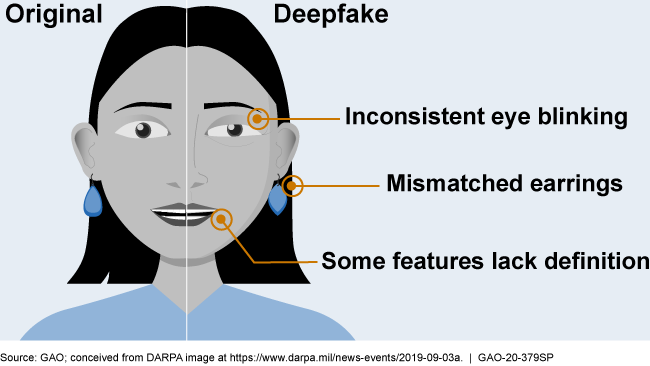
\includegraphics[width=0.9\textwidth]{images/rId14_image5.png}  
    \caption{Potential artifacts in a deepfake image or video (source: gao.gov)}  
    \label{figure:artifacts}  
\end{figure}  

Just as incoming email messages are analyzed for phishing attacks, and the attachments are scanned for viruses, images, audio, and videos may need to be scanned as well to aid the employee in detecting if they are genuine or deepfakes~\citep{mirsky_Creation_Detection_Deepfakes_2021}. Detecting deepfakes is a lot more computationally intensive than email phishing detection, so organizations may opt for giving employees the possibility of initiating a scan on material they suspect isn’t genuine.



Where once experts in the field could recommend that a caller be authenticated by recognizing their voice, accent, and intonations~\citep{mitnick_The_Art_of_Deception_2003}, with the advent of generative AI and especially deepfakes, this no longer holds true~\citep{doan_BTSE_Audio_Deepfake_Detection_2023}. Technologies such as the BTS-E encoder have been proposed for spotting idiosyncrasies in speech that might not or even could not be consciously registered by human observers, by detecting correlations between breathing, talking, and silence in calls and other audio.

%
% Seven deepfake artifacts
%
Seven different types of artifacts related to image and especially video deepfakes have been identified in two main categories~\citep{mirsky_Creation_Detection_Deepfakes_2021}: spatial-type artifacts which cover blending, environment, and forensics, while temporal-type artifacts cover behavior, physiology, synchronization, and coherence. Table \ref{table:deepfake_artifacts} explains these artifacts briefly.

\begin{table}[ht!]  
\centering
\renewcommand{\arraystretch}{1.5} % Adjust row height for better readability  
\setlength{\tabcolsep}{5pt} % Adjust column spacing  
\begin{tabularx}{\textwidth}{|l|l|X|} % X column for text wrapping  
\hline  
\textbf{Type} & \textbf{Artifact} & \textbf{Description} \\ \hline  
S & Blending & Related to the generated content when it is integrated back into a frame (the background), which is detectable with techniques such as edge detection and frequency analysis \\ \hline  
S & Environment & Appear when fake facial content seems inconsistent
with the surrounding background frame, often due to mismatches in warping, lighting, or
fidelity \\ \hline  
S & Forensics & Residues from the generative models, such as generative
adversarial network fingerprints or sensor noise \\ \hline  
T & Behavior & Relates to the monitoring of anomalies in the target’s mannerisms \\ \hline  
T & Coherence & Inconsistencies in logical sequences
happening over time\\ \hline  
T & Physiology & Inconsistencies in natural biological cues like blinking of
the eyes or head movements \\ \hline  
T & Synchronization & Mismatched
audio-visual elements \\ \hline  
\end{tabularx}  
\caption{Potential artifacts in deepfakes: S = spatial, T = temporal~\citep{mirsky_Creation_Detection_Deepfakes_2021}}  
\label{table:deepfake_artifacts}  
\end{table}  




\section{Education, pentests, and organizational changes}

User-oriented countermeasures against social engineering attacks usually fall into four broader categories~\citep{tsinganos_Towards_Automated_Recognition_Chat_SE_Enterprise_2018, mitnick_The_Art_of_Deception_2003}. These categories are simulated penetration tests with social engineering techniques, employee security awareness training programs, the creation and application of corporate cybersecurity policies, and the development of a security-conscious organizational culture.

Regular and comprehensive training programs are vital to educate employees about social engineering tactics. Regularity is stressed by experts in the field as users tend to forget what they have learned~\citep{hadnagy_Social_Engineering_The_Science_2018, mitnick_The_Art_of_Deception_2003}. It is thus suggested that training against social engineering attacks is not something that is done annually, or even bi-annually, but rather that it's something that is baked into the organization's culture. 

The inoculation theory~\citep{blauth_AI_Crime_Overview_Malicious_Use_Abuse_2022} suggests that prior exposure to social engineering attacks could help protect employees against future threats, whether these attacks are genuine or simulated. Conducting simulated social engineering and phishing attack campaigns (pentests, short for penetration testing), via numerous channels such as email, SMS, and even phone/VoIP, allows organizations to assess the susceptibility of their employees to social engineering tactics~\citep{hadnagy_Social_Engineering_The_Science_2018}. These exercises help identify vulnerabilities in the workforce, enabling further targeted training and reinforcing the importance of scrutinizing unsolicited communication, and with the advent of generative AI and deepfakes, this needs to be extended to received images, videos, and calls~\citep{mirsky_Creation_Detection_Deepfakes_2021}.

Employees should be shown what different varieties of deepfake content look like, as well as how easy it is to generate them~\citep{mirsky_Creation_Detection_Deepfakes_2021}. With the permission of the organization’s CEO or other top executives, their likeness could be used for this training material to add relevance.

It's imperative that every employee understands that they are the weakest link in the cybersecurity chain and that the responsibility for the organization's cybersecurity lies in everyone's hands, not just those of the cybersecurity professionals~\citep{mitnick_The_Art_of_Deception_2003}. If an employee has a user account in the organization’s systems, that is a potential entryway for threat actors. Due to the threat landscape widening, it's becoming increasingly vital to include more employee roles in cybersecurity training~\citep{ibm_Cost_Data_Breach_Report_2024}.

Finally, because AI can source social media sites and the Internet automatically for open-source intelligence, it's imperative for people to know to be careful of what they share, with whom and when~\citep{mitnick_The_Art_of_Deception_2003}. Even seemingly coincidental information, such as photos indicative that the employee is now on an organization-sponsored picnic, could be used against them and their employer in a social engineering attack.
